\chapter{Pollard-Rho para resolver ECDLP}
Em 1978, Pollard veio com o método Monte-Carlo\footnote{Monte-Carlo é um método estatístico que se baseiam em amostragens aleatórias massivas para obter resultados numéricos, isto é, repetindo sucessivas simulações um elevado número de vezes, para calcular probabilidades de forma heurística.} para resolver o problema do logaritmo discreto. Desde então, o método foi modificado para resolver o ECDLP. Como o algoritmo Pollard-Rho é atualmente o algoritmo mais rápido para resolver o ECDLP, então a segurança do ECC depende da eficiência desse algoritmo. Teoricamente, se o algoritmo Pollard-Rho é capaz de resolver o ECDLP eficientemente e em um tempo relativamente curto, então o criptossistema estará inseguro. \cite{Mandy:2007}

A estratégia do algoritmo é produzir uma sequência de termos gerados randomicamente $(R_k, a_k, b_k)$, onde \(R_k\) é um ponto na curva \(E\) e \(a_k\)  e \(b_k\) estão em $\mathbb{F}_p$ sobre a qual a curva elíptica \(E\) está definida. Como $E(\mathbb{F}_p)$ é um grupo finito, a sequência eventualmente irá torna-se periódica e voltará para um termo anterior da sequência. Usa-se essa periodicidade para resolver ECDLP. Como nem sempre a sequência volta para o primeiro termo, um diagrama da sequência parecerá com a letra Grega \(\rho\) (Ver figura \ref{fig:rho}). Por este motivo esse método é chamado de Pollard-Rho. Essa sequência de termos gerados é chamada de ``percurso''.

Seja \(\mu\) o tamanho da calda e \(\lambda\) o tamanho do ciclo. Após um número finito de iterações, obtêm-se os termos $R_k = R_{k+\lambda}$, onde $k > \mu$ e $\lambda > 1$. Neste ponto, já deverá ter sido encontrado uma correspondência entre os termos e poderá aplicar matemáticas discretas para resolver os problemas de logaritmo discreto gerado pelos elementos do conjunto finito.

A seguir serão apresentados o algoritmo de Pollard-Rho e suas variações.

\begin{figure}[h]
\centering
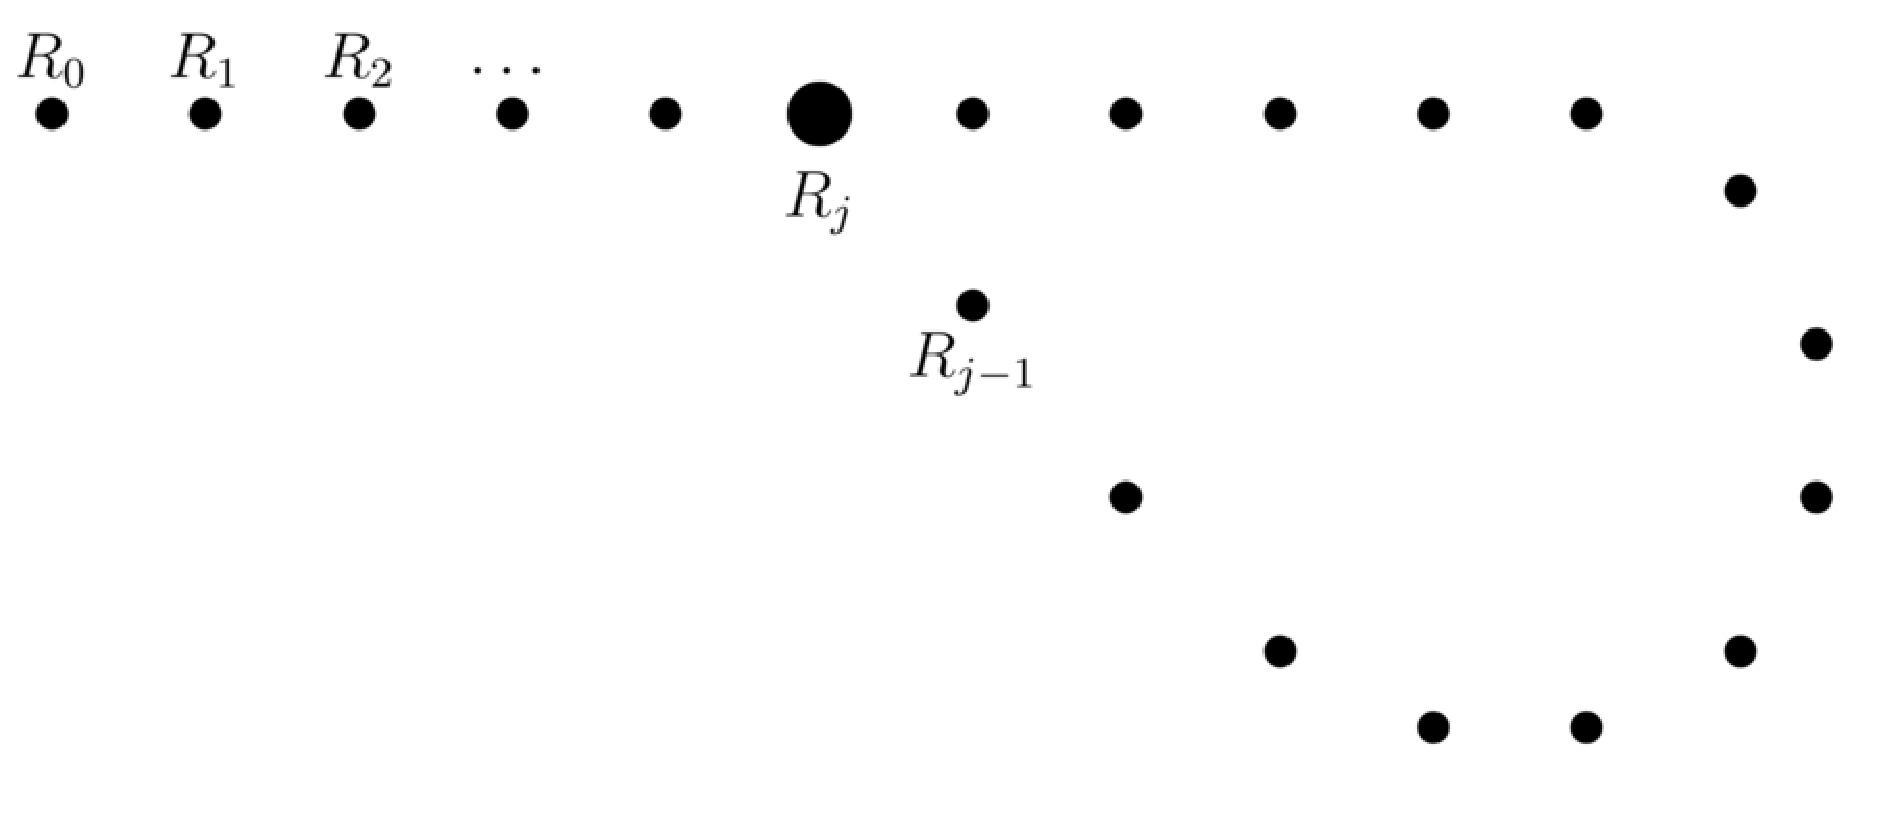
\includegraphics[scale=0.4, bb=0 0 888 376]{figuras/rho.eps}
\caption{Diagrama da sequência produzida pelo algoritmo Pollard-Rho}
\label{fig:rho}
\end{figure}

\section{Pollard-Rho original}
Seja $G = E(\mathbb{F}_p)$, tal que a ordem de $G = n$, e \(P\) e \(Q\) tal que $Q = xP$ em \(G\). O objetivo é calcular \(x\). Segue os passos:

\begin{enumerate}
\item \(G\) é particionado em 3 conjuntos $S_1, S_2, S_3$ de aproximadamente do mesmo tamanho, em que $\mathcal{O} \notin S_2$.
\item Definir uma função de iteração $f : R \to R$ de um percurso aleatório:

\begin{eqnarray} \label{eq:walk}
R_{k+1} = f(R_k) =
\begin{cases}
Q + R_k, &R_k \in S_1 \\
2R_k, &R_k \in S_2 \\
P + R_k, &R_k \in S_3
\end{cases}
\end{eqnarray}

\item Seja $R_k = a_kP + b_kQ$, e portanto

\begin{eqnarray}
a_{k+1} =
\begin{cases}
a_k, &R_k \in S_1 \\
2a_k \pmod n, &R_k \in S_2 \\
a_k + 1, &R_k \in S_3
\end{cases}
\end{eqnarray}

e

\begin{eqnarray}
b_{k+1} =
\begin{cases}
b_k + 1, &R_k \in S_1 \\
2b_k \pmod n, &R_k \in S_2 \\
b_k, &R_k \in S_3
\end{cases}
\end{eqnarray}

\item Os termos iniciais são: $R_0 = P, a_0 = 1, b_0 = 0$ e os pares gerados $(R_k, R_{2k})$ até encontrar uma correspondência $R_m = R_{2m}$, para qualquer \(m\).

\item Uma vez encontrados, calcule:

\begin{eqnarray*}
R_m = a_mP + b_mQ \\
R_{2_m} = a_{2_m}P + b_{2m}Q
\end{eqnarray*}

\item Com isso, é possível calcular \(x\):

\begin{equation} \label{eq:x}
x = (a_{2m} - a_m)(b_m - b_{2m})^{-1} \pmod n
\end{equation}

\end{enumerate}

O termo $(b_m - b_{2m})^{-1}$ em \ref{eq:x} somente é possível calcular quando o GCD$(b_m - b_{2m}, n) = 1$, ou seja, quando \(b_m\) e \(b_{2m}\) são coprimos entre si. Caso contrário, o algoritmo não poderá continuar.

\section{Pollard-Rho com único processador}
Este algoritmo segue a idéia do Pollard-Rho original, no entanto, a abordagem se diferencia na escolha aleatória de parâmetros e menor utilização de armazenamento de memória \cite{Guide}.

% #INPUT: Curva elipitica E e Pontos P e Q $\in$ E
% #OUTUPT: x = $\log_P$ Q

\begin{lstlisting}[caption={Algoritmo Pollard-Rho com único processador.},label=single]
pollardRho_singleProcessor(E: Curva, P: Ponto, Q: Ponto): inteiro
	seja L, n, inteiro
	seja cn, dn, inteiro
	seja cm, dm, inteiro
	seja Xn, Xm, Ponto
	seja a, b, R, array

	n := E.ordem()
	para j := 1, enquanto j <= L, faca
		a[j] := random() % n
		b[j] := random() % n
		R[j] := a[j]*P + b[j]*Q

	cn := random() % n
	dn := random() % n
	Xn := cn*P + dn*Q
	cm := cn
	dm := dn
	Xm := Xn

	enquanto Xn != Xm faca
		j := H(Xn)
		Xn := Xn + R[j]
		cn := cn + a[j]
		dn := dn + b[j]

	se dn = dm entao
		retorne "falha"

	seja x, inteiro
	x := (cn - cm)/(dm - dn) % n
	retorne x

H(P: Ponto): inteiro
	retorne P.x % 4 + 1

\end{lstlisting}

Assumindo que o percurso aleatório \ref{eq:walk} definido no algoritmo produz termos aleatórios, então a primeira colisão na sequência é esperada para após $\sqrt{\pi n/2}$ termos. Além disso, o tamanho da calda prevista é de $\mu \approx \sqrt{\pi n/8}$ e o tamanho do ciclo $\lambda \approx \sqrt{\pi n/8}$ \cite{Pollard:1978}. Isso implica que o número de termos gerados até encontrar uma correspondência é proporcional à raiz quadrada da ordem da curva.

